As I told in the Abstract, the main objective of this experience was the
installation of the \PTP\ daemon on the \MyBoard. The installation
procedure I described till now it's pretty general, while in this section
I'll focus on the protocol itself.

\subsection{ The software }

    The two applications can be easily cross compiled once you are
    provided with a working cross-compiler, as explained in
    section~\ref{sec:GetTools}.

    \subsubsection{ \PTPd\ hosted by \SourceForge }

        The \Const{2.1.0} version of the original project, henceforth
        referred as \PTPd) is hosted by \SourceForge\ at
        \url{http://ptpd.sourceforge.net/}. It can be cross-compiled
        in a seamless and straightforward way:
\begin{lstlisting}
    host$ cd ptpd-2.1.0/src/

    host$ CC=powerpc-linux-gcc make
    powerpc-linux-gcc -c -Wall   -o ptpd.o ptpd.c
    powerpc-linux-gcc -c -Wall   -o arith.o arith.c
    powerpc-linux-gcc -c -Wall   -o bmc.o bmc.c
    powerpc-linux-gcc -c -Wall   -o protocol.o protocol.c
    powerpc-linux-gcc -c -Wall   -o display.o display.c
    powerpc-linux-gcc -c -Wall   -o dep/msg.o dep/msg.c
    powerpc-linux-gcc -c -Wall   -o dep/net.o dep/net.c
    powerpc-linux-gcc -c -Wall   -o dep/servo.o dep/servo.c
    powerpc-linux-gcc -c -Wall   -o dep/startup.o dep/startup.c
    powerpc-linux-gcc -c -Wall   -o dep/sys.o dep/sys.c
    powerpc-linux-gcc -c -Wall   -o dep/timer.o dep/timer.c
    powerpc-linux-gcc -lm -lrt -o ptpd2 ptpd.o arith.o bmc.o protocol.o
    display.o dep/msg.o dep/net.o dep/servo.o dep/startup.o dep/sys.o
    dep/timer.o

    host$ file ptpd2
    ptpd2: ELF 32-bit MSB executable, PowerPC or cisco 4500, version 1
    (SYSV), dynamically linked (uses shared libs), for GNU/Linux 2.4.3,
    not stripped
\end{lstlisting}

        In the uploading step (you may use the methods described in
        Sections \ref{sec:Upload} and \ref{sec:UploadImages}) you can
        simply activate the daemon just after the bootstrap phase (see
        Section~\ref{sec:HackImages}).

        In order to quickly test the functionality of the daemon, after
        plugging it into the \emph{Master}, I tried to:
        \begin{itemize}
        \item   Deactivate the daemon (by using the \Command{kill}
                command);
        \item   Set a random date on the board (by using the \Command{date}
                command);
        \item   Reactivate the daemon (just by launching it).
        \end{itemize}
        The date immediately synchronized with the \emph{Master}, and this
        is a nice proof of concept, although not exhaustive: accurate
        statistics are needed.
        The daemon provides a way to obtain such data. More on this on
        Subsection~\ref{sub:Stats}.

        \Note{Lack of hardware support}{
            This project is just a user-space software implementation of
            the \PTP\ protocol. In order to enable the \Vitesse\ device a
            kernel-space support is needed. The fork hosted by
            \GoogleCode\ provides a \Linux\ kernel module.  See
            Subsection~\ref{subsub:PTPdV2}.
        }

    \subsubsection{ \PTPd\ hosted by \GoogleCode } \label{subsub:PTPdV2}

        This is a forked project, derived from the \emph{rc1} version of
        \PTPd, and in this document I will refer to it as \PTPdGC. It's
        hosted by \GoogleCode\ at \url{http://code.google.com/p/ptpv2d/}.

        In this case the compilation process is tainted by a good amount
        of syntax errors and warnings. Since they can be easily fixed
        without knowing anything on the program logic, it's probable
        they'll be removed on the next release. At any rate you can find a
        patch covering the problem in the \MyRepo\ (see
        Subsection~\ref{sub:Resources}). The patch can be applied as
        follows:
\begin{lstlisting}
  host$ cd ptpv2d-dev

  host$ patch -p1 < Path-to-repo/patches/ptpv2d-dev-compile.patch
  patching file application/src/arith.c
  patching file application/src/dep/constants_dep.h
  patching file application/src/dep/net.c
  patching file application/src/protocol.c
\end{lstlisting}

        At this point the compilation process of the application just
        requires a call to \Command{make}:
\begin{lstlisting}
  host$ cd application/src

  host$ CC=powerpc-linux-gcc make
  powerpc-linux-gcc -c -Wall -DPTPD_DBGV -Dlinux -DSOCKET_TIMESTAMPING
  -o ptpv2d.o ptpv2d.c
  ...
  ...
  ...
  powerpc-linux-gcc -c -Wall -DPTPD_DBGV -Dlinux -DSOCKET_TIMESTAMPING
  -o dep/ledlib.o dep/ledlib.c
  powerpc-linux-gcc -lrt -o ptpv2d ptpv2d.o arith.o bmc.o probe.o
  protocol.o v2utils.o v2bmc.o dep/msg.o dep/net.o dep/servo.o
  dep/startup.o dep/sys.o dep/timer.o dep/ledlib.o

  host$ file ptpv2d
  ptpv2d: ELF 32-bit MSB executable, PowerPC or cisco 4500, version 1
  (SYSV), dynamically linked (uses shared libs), for GNU/Linux 2.4.3,
  not stripped
\end{lstlisting}

        Also note that this project provides a \Linux\ kernel module that
        allows the daemon to be interfaced with the \Vitesse\ device,
        although I didn't try it.

\subsection{ Getting statistics } \label{sub:Stats}

    As explained, the two softwares are rooted in the same project, thus
    they've got some common part. One of those is the logging system. Both
    software support two options for logging: the first one is \Const{-d},
    which produces the output in a binary format, the second one is
    \Const{-D}, which produces a \StdName{comma separated value} output.

    \subsection{ Transmitting statistics }

        Of course parsing the board statistics on the board itself is not
        a good idea. It's useful to send the data to the host. This can be
        easily achieved by using \NetCat\ as we did in
        Section~\ref{sec:Upload}. Two steps are needed:
        \begin{enumerate}
        \item   Start a listening server on the host
\begin{lstlisting}
    host$ nc -l -p 9001 > data/stats.txt
\end{lstlisting}
        \item   Restart the daemon and send the output on the server
\begin{lstlisting}
    board$ killall ptpd2
    board$ /sbin/ptpd2 -D | nc <host-ip-addr> 9001 &
\end{lstlisting}
        \end{enumerate}
        This procedure doesn't depend on the software we run, so
        you can do it for both the versions of the daemon.

    \subsection{ Parsing statistics of \PTPd }

        This is a sample of the output of the daemon:
\begin{lstlisting}
  host$ head -n 6 data/stats.txt
  timestamp, state, clock ID, one way delay, offset from master, slave
  to master, master to slave, drift
  2011-07-27 13:54:59:468577, init
  2011-07-27 13:54:59:469608, lstn
  2011-07-27 13:55:00:047391, slv, 0050c2fffed28deb/01, 0.000000000,
  0.000000000, 0.000000000, 0.000000000, 0
  2011-07-27 13:55:01:036986, slv, 0050c2fffed28deb/01, 0.000000000,
  -0.000635995, 0.000000000, 0.001271990, -635
  2011-07-27 13:55:02:198700, slv, 0050c2fffed28deb/01, 0.000000000,
  -0.001267090, 0.000000000, 0.001262190, -1902
\end{lstlisting}

        I found on the web a \TechName{Python} script which was supposed
        to convert the \StdName{csv} to some input suitable for
        \TechName{gnuplot}, but it was pretty awkward to use, so I decided
        to restyle it, ending up in rewriting it from scratch using
        \TechName{PyLab}. You can find it in my \MyRepo\ (the file is
        \FileName{programs/ptpd-parse}).

\newpage
        \subsubsection{Simple usage of \TechName{ptpd-parse}}

            The simplest way of using it is just redirecting the \emph{log
            file} as standard input for the script:
\begin{lstlisting}
  host$ cat data/stats.txt | programs/ptpd-parse
\end{lstlisting}
            which will show two windows:
            \begin{itemize}
            \item   The first one (\emph{figure 1}) will contain the time
                    evolution of:
                \begin{itemize}
                \item   \emph{One way delay};
                \item   \emph{Offset from Master};
                \item   \emph{Slave to Master};
                \item   \emph{Master to Slave};
                \end{itemize}
            \item   The second one (\emph{figure 2}) will contain the time
                    evolution of the \emph{Time drift};
            \end{itemize}

        \subsubsection{Parameters of \TechName{ptpd-parse}}

            The \Const{--help} flag will display the inline help:
\begin{lstlisting}
  host$ ./programs/ptpd-parse --help

  Usage: ptpd-parse [options]

  Options:
    -h, --help          show this help message and exit
    --one-way-delay=ONE_WAY_DELAY
                        Select window for one-way-delay (default: 1)
    --offset-from-master=OFFSET_FROM_MASTER
                        Select window for offset-from-master
    --slave-to-master=SLAVE_TO_MASTER
                        Select window for slave-to-master (default: 1)
    --master-to-slave=MASTER_TO_SLAVE
                        Select window for master-to-slave (default: 1)
    --time-drift=TIME_DRIFT
                        Select window for time draft (default: 2)
    -l LOGFILE, --logfile=LOGFILE
                        Log file (default: stdin)
    -o OUT_FORMAT, --out=OUT_FORMAT
                        Output file format (default: show window)
    --out-fname=OUT_FILENAME
                        Output file name (default:"figure")
\end{lstlisting}

            By selecting windows you can decide where to plot data. For
            instance, the following command will plot the \emph{One way
            delay} and the \emph{Offset from Master} in a window,
            the \emph{Slave to Master} and the \emph{Master to Slave} into
            another window, and won't display the \emph{Time drift}.
\begin{lstlisting}
  host$ cat data/stats.txt | programs/ptpd-parse --one-way-delay=1
    --offset-from-master=1 --slave-to-master=2 --master-to-slave=2
    --time-drift=0
\end{lstlisting}

            Also you can save the plots on output files. You can specify a
            format with the \Const{--out} or \Const{-o} flag. For instance
            the following command is like the previous one, but saves
            the \emph{One way delay} and the \emph{Offset from Master} in
            a file named \FileName{figure01.pdf}, the \emph{Slave to
            Master} and the \emph{Master to Slave} into a file named
            \FileName{figure02.pdf}, and won't save the \emph{Time
            drift}:
\begin{lstlisting}
  host$ cat data/stats.txt | programs/ptpd-parse --one-way-delay=1
    --offset-from-master=1 --slave-to-master=2 --master-to-slave=2
    --time-drift=0 --out=pdf
\end{lstlisting}
            If you don't like the name \FileName{figure01.pdf} and you
            prefer \FileName{garbage.pdf} try with the
            \Const{--out-fn=garbage} option.

\subsection{ Example of statistics }

    Here there are some examples of statistics I collected during my
    experiments. Unfortunately they are not so significative, but still
    they give an idea of the kind of data resulting from the daemon's
    output log.

    In order to test the system I tried to connect the board with a Master
    through a \StdName{RJ-45} cable, then I activated the daemon on the
    board as explained in Subsection~\ref{sub:Stats}, collecting
    statistics relative to the board on a file.

    Figure~\ref{img:OFM-MTS} shows the evolution of the \emph{system time
    offset} with respect to the Master (in cyan) and the time required by
    the synchronization signal produced by the Master to reach the board
    (Magenta). The graphic in Figure~\ref{img:TimeDrift}, on the other
    hand, shows the behavior of the Slave's time drift in the same period.

    \begin{figure}[p]
        \centering
        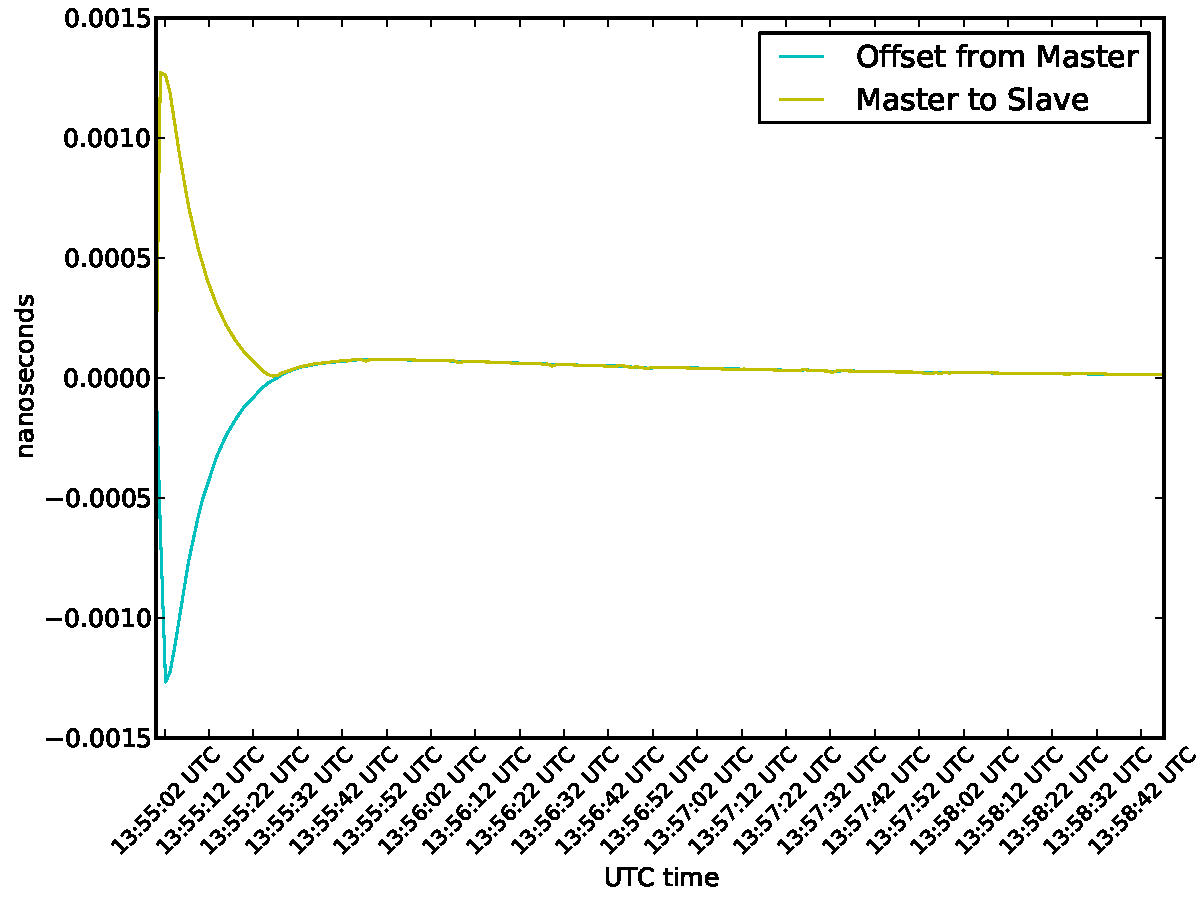
\includegraphics[width=.8\textwidth]{pics/figure01}
        \caption{Data sample collected by the board: \emph{Offset from
                 Master} and \emph{Master to Slave}}
        \label{img:OFM-MTS}
    \end{figure}

    \begin{figure}[p]
        \centering
        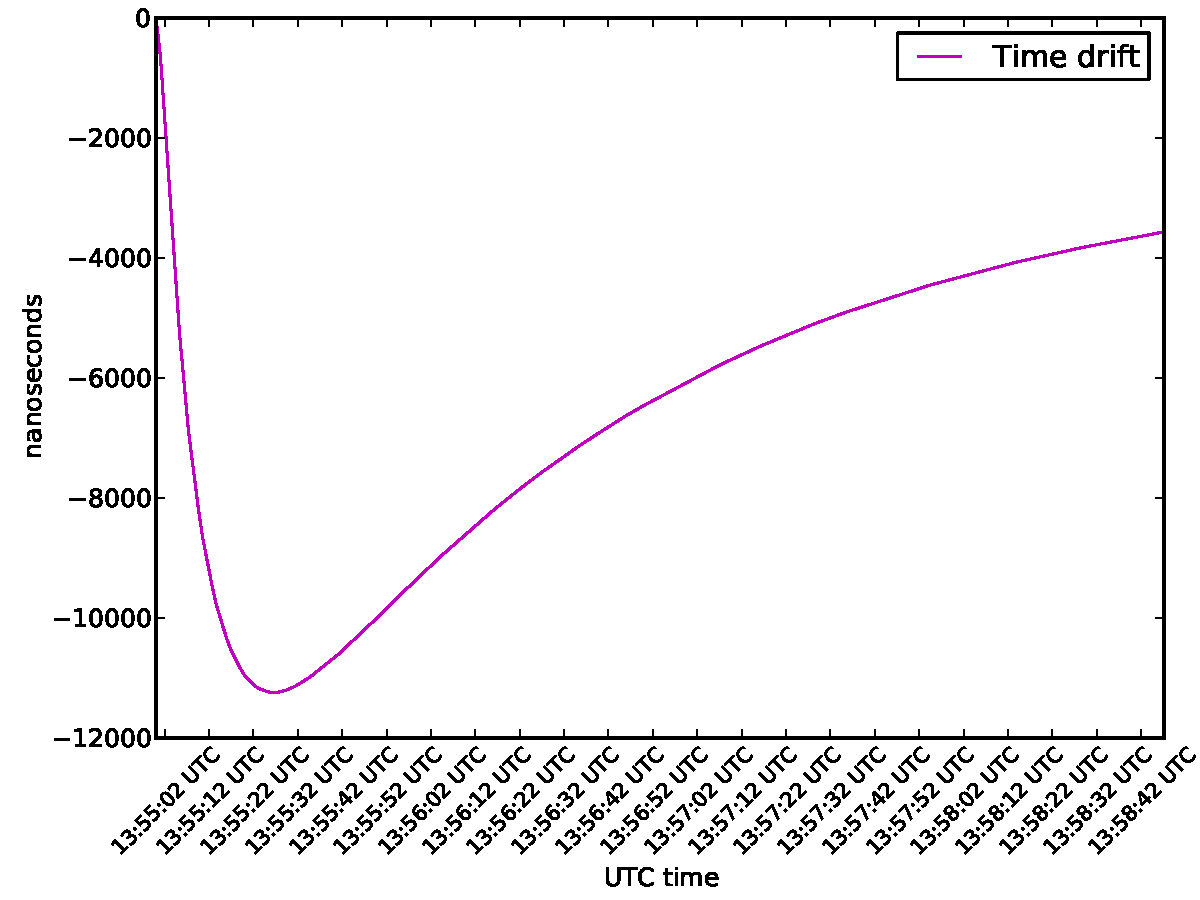
\includegraphics[width=.8\textwidth]{pics/figure02}
        \caption{Data sample collected by the board: \emph{Time drifting}
                 of the Slave's clock}
        \label{img:TimeDrift}
    \end{figure}

